\documentclass{article}

\usepackage{amsmath}
\usepackage{amsfonts} % For math fonts.
\usepackage{amssymb} % For other math symbols not covered by amsmath.
\usepackage[pdftex]{graphicx} % For pictures, use %\includegraphics[scale=decimal]{pic.png}; must be a .png file type.
\usepackage{multicol}
\usepackage{textcomp}
\usepackage[colorlinks = true, urlcolor = blue]{hyperref}
\usepackage{enumitem}
\usepackage{graphbox} 
\usepackage{subfig}
\usepackage{multicol}

\newcommand{\tab}{\hspace*{0.25in}}

\usepackage{tikz}
\usetikzlibrary{positioning, calc}
\usetikzlibrary{shapes.geometric,angles,quotes}
\usepackage{tikz-3dplot}

\newcommand{\csq}[1]{\reflectbox{''}#1''}  %This produces CS style quotes.



\usepackage{fullpage}
\usepackage{listings}
\lstset
{ %Formatting for code in appendix
    language=Python,
    basicstyle=\footnotesize,
	%keywordstyle=\color{blue}\bfseries, % Styles keywords (e.g., def, import)
	%commentstyle=\color{green}\itshape, % Styles comments
    numbers=left,
    stepnumber=1,
    showstringspaces=false,
    tabsize=2,
    breaklines=true,
    breakatwhitespace=false,
%    escapechar=\n
}


\begin{document}


\begin{flushright}
Debugging\end{flushright}

\vspace*{-1.5em}
\noindent\makebox[\linewidth]{\rule{\paperwidth}{0.4pt}}


\vspace*{2em}

\begin{enumerate}

%standard 10.1

%start_of_questions


%new_question
%%%%%%%%%%%%%%%%%%%%%
	% Problem 1
	% Difficulty: 1
%%%%%%%%%%%%%%%%%%%%%
	\item 
		In Harry Potter, the currency consists of knuts, sickle, and galleon. There are 29 knuts in 
		one sickle and 17 sickles in one galleon. Write a \textbf{function} that will return a 
		converted amount of knuts into the fewest amount of coins possible. Only return a string 
		with the non-zero values, meaning don't return something similar to ``0 sickles''. The 
		argument for the function will be $knuts$ (how many knuts to convert), if no argument is 
		provided then the \textbf{default} should be 900 knuts. \\ \\
		\textbf{Debug this Solution:}\\
		\mbox{ \hspace*{0.25in}	\lstinputlisting[language=Python]{./code/debugger_p1_HarryPotter.py}}

%Error 1: default should be 900
%Error 2: remaining_knuts should use remainder \% not //
%Error 3: first if for galleons should be >
\pagebreak



%new_question
%%%%%%%%%%%%%%%%%%%%%
	% Problem 2
	% Difficulty: 1
%%%%%%%%%%%%%%%%%%%%%
	\item 
		Primary U.S. interstate highways are numbered 1-99 (Inclusive).  Odd numbers (like 5 or 95) go north/
		south, and evens (like 10 or 82) go east/west.  Auxiliary highways are numbered 100-999, and 
		service the primary highway indicated by the rightmost two digits.  Thus, I-405 services 
		I-5, and I-290 services I-90.
		
		Note: 200 is not a valid auxiliary highway because 00 is not a valid primary highway 
		number.\\
		
		Write a \textbf{function} that returns whether the highway runs north/south or east/west or is an 
		invalid highway number. The argument for the function 
		will be $highway\_num$(highway number provided). \\ \\
		\textbf{Debug this Solution:}\\
		\mbox{ \hspace*{0.25in}	\lstinputlisting[language=Python]{./code/debugger_p2_HighwayDirections.py}}

% Error 1: "if 1 > highway_num < 99" should be "if 1 <= highway_num <= 99"
% Error 2: In primary highways, the return strings for even/odd are swapped.
% Error 3: In the auxiliary highway service check, 'elif' should be 'else' because it incorrectly checks the same condition twice.
\pagebreak



%new_question
%%%%%%%%%%%%%%%%%%%%%
	% Problem 3
	% Difficulty: 1
%%%%%%%%%%%%%%%%%%%%%
	\item 
		%https://edabit.com/challenge/xR248CxGSsSrNK5Za
		You are the newest rug fashion designer on the scene, but you're running out of ideas. 
		Write a \textbf{function} that will help you design rugs.  The function will return a 
		formatted string that will resemble a designed rug. The first parameter must be $width$ 
		(how wide the rug will be), the second must be $length$ (how long the rug will be), 
		and the third must be $pattern$ (the character pattern used in the rug design).

		\textbf{Examples:} \\
			design\_run(3,5,\$) $\rightarrow$	\begin{tabular}{l}
			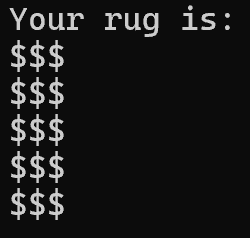
\includegraphics[height=1in]{./imgs/rug1_alt.PNG} \hspace{0.5in} \end{tabular}
			design\_run(16,5,\@) $\rightarrow$ \begin{tabular}{l}
			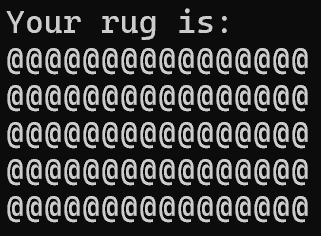
\includegraphics[height=1in]{./imgs/rug2_alt.PNG} \end{tabular}

		\textbf{Debug this Solution:}\\
		\mbox{ \hspace*{0.25in}	\lstinputlisting[language=Python]{./code/debugger_p3_Rugs.py}}

%Error 1: for i in range(length -1) should be for i in range(length)
%Error 2: pattern should be pattern ='@'
%Error 3: result += "\t" should be result += "\n"
\pagebreak



%new_question
%%%%%%%%%%%%%%%%%%%%%
	% Problem 4
	% Difficulty: 1
%%%%%%%%%%%%%%%%%%%%%
	\item 
		%https://edabit.com/challenge/b8wRDMWgMZTN2nmfx
		Write a \textbf{function} that returns the number of copies of the same number. 
		The arguments for the function will be $num\_1$ (first number), $num\_2$ (second number), 
		and $num\_3$ (third number).\\

		\textbf{Examples:}		
		\begin{itemize}
			\item  count\_duplicates(2, 3, 2) $\rightarrow$ \csq{You entered the same number 2 times}, 
			\item  count\_duplicates(4, 4, 4) $\rightarrow$ \csq{You entered the same number 3 times}, 
			\item  count\_duplicates(1, 2, 3) $\rightarrow$ \csq{Each number is unique} 
		\end{itemize}

		\textbf{Debug this Solution:}\\
		\mbox{ \hspace*{0.25in}	\lstinputlisting[language=Python]{./code/debugger_p4_NumberCopies.py}}

%Error 1: count should be 1
%Error 2: count = 1 should be count += 1
%Error 3: num_1 == num_3 is repeated twice
\pagebreak




%new_question
%%%%%%%%%%%%%%%%%%%%%
	% Problem 6
	% Difficulty: 1
%%%%%%%%%%%%%%%%%%%%%
	\item
		Write a function called \textit{flip\_flop} that takes a string as an argument 
		and returns a new word made up of the second half of the word first combined 
		with the first half of the word second.\\ 

		\textbf{Debug this Solution:}\\
		\mbox{ \hspace*{0.25in}	\lstinputlisting[language=Python]{./code/debugger_p6_FlipFlop.py}}

%Error 1: if length // 2 == 0: should be if length % 2 == 0:
%Error 2: first_half = word[middle:] should be first_half = word[:middle]
\pagebreak



%new_question
%%%%%%%%%%%%%%%%%%%%%
	% Problem 7
	% Difficulty: 1
%%%%%%%%%%%%%%%%%%%%%
	\item 
		The hamming distance is the number of characters that differ between two strings. 
		Write a function named hamming\_distance that takes two strings as arguments and 
		returns the hamming distance.\\
		
		\textbf{Debug this Solution:}\\
		\mbox{ \hspace*{0.25in}	\lstinputlisting[language=Python]{./code/debugger_p7_HammingDistance.py}}

%Error 1: distance = 1 should be distance = 0
%Error 2: for i in range(len(str1) -1): should be for i in range(len(str1) ):
%Error 3: if str1[i] == str2[i]: should be if str1[i] != str2[i]:
\pagebreak


%end_of_questions
%make sure to leave at least one blank line below


%standard 10.2


%start_of_questions


%new_question
%%%%%%%%%%%%%%%%%%%%%
	% Problem 8
	% Difficulty: 1
%%%%%%%%%%%%%%%%%%%%%
	\item 
		Given a positive integer $n$, the following rules will always create a sequence that 
		ends with 1, called Hailstone Sequence:
		\begin{enumerate}
			\item If $n$ is even, divide by 2
			\item If $n$ is odd, multiply by 3 and add 1 (i.e. $3n+1$)
			\item Continue until $n$ is 1
		\end{enumerate}
		Write a \textbf{function} that returns a list with the hailstone sequence starting at $n$. 
		The argument to the function will be $n$ (the integer to start the sequence from).\\

		\textbf{Debug this Solution:}\\
		\mbox{ \hspace*{0.25in}	\lstinputlisting[language=Python]{./code/debugger_p9_HailstoneSequence.py}}

%Error 1: n/n should be n
%Error 2: sequence.append(n) should have an extra indentation
%Error 3: while n == 1 should be while != 1
\pagebreak



%new_question
%%%%%%%%%%%%%%%%%%%%%
	% Problem 9
	% Difficulty: 1
%%%%%%%%%%%%%%%%%%%%%
	\item
		YouTube currently displays a like and a dislike button, allowing you to express your opinions 
		about particular content. 
		It's set up in such a way that you cannot like and dislike a video at the same time.
		There are two other interesting rules to be noted about the interface:
		\begin{enumerate}
			\item Pressing a button, which is already active, will undo your press.
			\item If you press the like button after pressing the dislike button, the like button overwrites 
				the previous \csq{dislike} state. The same is true for the other way round.
		\end{enumerate}
		Write a \textbf{function} that takes in a list of button inputs $events$ and returns the final state.\\

		\textbf{Debug this Solution:}\\
		\mbox{ \hspace*{0.25in}	\lstinputlisting[language=Python]{./code/debugger_p10_YouTube.py}}

%Error 1: initial state = "like" should be state = "nothing"
%Error 2: for event in range(events) should be for event in events
%Error 3: if event != state: should be if event == state:
\pagebreak



%new_question
%%%%%%%%%%%%%%%%%%%%%
	% Problem 10
	% Difficulty: 1
%%%%%%%%%%%%%%%%%%%%%
	\item 	
		%https://edabit.com/challenge/yL5WmWTCNwwb4GnR7
		In each input list, every number repeats at least once, except for two. Write a \textbf{function} 
		that takes an array $numbers$ and returns the two unique numbers.\\

		\textbf{Debug this Solution:}\\
		\mbox{ \hspace*{0.25in}	\lstinputlisting[language=Python]{./code/debugger_p11_TwoUniqueNumbers.py}}

%Error 1: for num in range(len(numbers)) should be for num in numbers
%Error 2: code in if and else statements should be swapped.
%Error 3: number_dicitonary.values() should be number_dicitonary
\pagebreak



%new_question
%%%%%%%%%%%%%%%%%%%%%
	% Problem 11
	% Difficulty: 1
%%%%%%%%%%%%%%%%%%%%%
	\item 
		%https://edabit.com/challenge/6Pf5GGG6HnzbB95gf
		Write a \textbf{function} that returns a list with the factors of a given integer. 
		The argument of the function will be $num$ (integer to find factors for).\\

		\textbf{Debug this Solution:}\\
		\mbox{ \hspace*{0.25in}	\lstinputlisting[language=Python]{./code/debugger_p13_Factors.py}}

%Error 1: for i in range(1, num): should be for i in range(1, num+1):
%Error 2:  if num % i != 0: should be if num % i == 0:
%Error 3: factors.add(i) should be factors.append(i)
\pagebreak




%new_question
%%%%%%%%%%%%%%%%%%%%%
	% Problem 12
	% Difficulty: 1
%%%%%%%%%%%%%%%%%%%%%
\item
	Write a \textbf{function} that takes a list of words $words$ and returns a dictionary where 
	the keys categorize words based on whether they are palindromes. 
	The categories are defined as follows:
	\begin{enumerate}  
		\item \csq{Palindrome} includes words that read the same forward and backward.  
		\item \csq{Non-palindrome} includes all other words.  
	\end{enumerate}  

		\textbf{Debug this Solution:}\\
		\mbox{ \hspace*{0.25in}	\lstinputlisting[language=Python]{./code/debugger_p14_Palindromes.py}}

%Error 1: reduce indent of if and else
%Error 2: put "reversed_word = ' ' '' inside first loop
%Error 3: switch content of if and else OR change if statement from == to !=
\pagebreak



%new_question

%%%%%%%%%%%%%%%%%%%%%
	% Problem 13
	% Difficulty: 1
%%%%%%%%%%%%%%%%%%%%%
	\item
		(Game: Odd or Even)  Write a \textbf{function} that lets the user guess whether a randomly 
		generated number is odd or even.  The function randomly generates an integer between 0 and 9 
		(inclusive) and returns whether the user's guess is correct or incorrect. The argument for 
		the function will be $guess$ (the user's guess, either \csq{odd} or \csq{even}), if no 
		argument is provided then the \textbf{default} guess should be even.\\
		Hint: Use the following lines of code to create the function.
		\begin{verbatim}
		    from random import randint
		    value = randint(0,9) #picks a random integer between 0-9 inclusive
		\end{verbatim}

		\textbf{Debug this Solution:}\\
		\mbox{ \hspace*{0.25in}	\lstinputlisting[language=Python]{./code/debugger_p15_EvenOrOdd.py}}


%Error 1: from random import randominteger should be from random import randomint
%Error 2: def guess(guess="odd"): should be def guess(guess="even"):
%Error 3: if value // 2 == 0: should be if value % 2 == 0:
\pagebreak


%end_of_questions
%make sure to leave at least one blank line below



\end{enumerate}
\end{document}



%new_question
%%%%%%%%%%%%%%%%%%%%%
	% Problem 8
	% Difficulty: 1
%%%%%%%%%%%%%%%%%%%%%
	\begin{minipage}{.6\textwidth}
		\item Create a \textit{Recipe} class.\\
		A \textit{Recipe} has
		\begin{itemize}
			\item name 
			\item cooking\_time
			%\item calores\_per\_serving
		\end{itemize}

		A \textit{Recipe} can do
		\begin{itemize}
			\item is\_quick\_meal
			%\item calculate\_calories\_total(servings)
		\end{itemize}
	\end{minipage}
		%
	\begin{minipage}{.4\textwidth}
		This class ``looks'' like 
				
		\vspace*{1em}
		\begin{tabular}{|l|}
			\hline Circle\\ \hline
			name\\ cooking\_time \\  \hline
			is\_quick\_meal\\ \hline
		\end{tabular}
	\end{minipage}

	\vspace*{2ex}
	Create a constructor method that initializes all instance variables.\\
	You should write getters and setters for each of the instance variables.\\
	Instantiate an instance of the class. You may pass any initial values of your choosing.	

	The is\_quick\_meal() method should return True if the cooking\_time is less than 30 minutes and False 
	if it takes 30 minutes or more.\\
		
		\textbf{Debug this Solution:}\\
		\mbox{ \hspace*{0.25in}	\lstinputlisting[language=Python]{./code/debugger_p8_RecipeClass.py}}

%Error 1: def __init__(name, cooking_time): should be def __init__(self, name, cooking_time):
%Error 2: return cooking_time should be return self.cooking_time
%Error 3: return self.cooking_time == 30 should be return self.cooking_time < 30
\pagebreak




%new_question
%%%%%%%%%%%%%%%%%%%%%
	% Problem 12
	% Difficulty: 1
%%%%%%%%%%%%%%%%%%%%%
	\begin{minipage}{.6\textwidth}
	\item Create a \textit{Vector} class.\\
		A \textit{Vector} has
		\begin{itemize}
			\item x\_direction 
			\item y\_direction
		\end{itemize}
		
		A \textit{Vector} can do
		\begin{itemize}
			\item get\_magnitude
		\end{itemize}
	\end{minipage}
		%
	\begin{minipage}{.4\textwidth}
		This class ``looks'' like 
				
		\vspace*{1em}
		\begin{tabular}{|l|}
			\hline Vector\\ \hline
			x\_direction\\ y\_direction\\ \hline
			get\_magnitude\\  \hline
		\end{tabular}
	\end{minipage}

	\vspace*{2ex}
	Create a constructor method that initializes all instance variables.\\
	You should write getters and setters for each of the instance variables.\\
	Instantiate an instance of the class. You may pass any initial values of your choosing.
	
	Hint: magnitude is calculated as $\sqrt{x^2 + y^2}$.

		\textbf{Debug this Solution:}\\
		\mbox{ \hspace*{0.25in}	\lstinputlisting[language=Python]{./code/debugger_p12_Vector.py}}

%Error 1: def __init__(x_direction, y_direction): should be def __init__(self, x_direction, y_direction):
%Error 2: return self.y_direction should be return self.x_direction
%Error 3: sqrt should be math.sqrt and import math OR from math import sqrt
\pagebreak



%new_question
%%%%%%%%%%%%%%%%%%%%%
	% Problem 5
	% Difficulty: 1
%%%%%%%%%%%%%%%%%%%%%
	\item Create a \textit{ColorRGB} class.
	
	\begin{minipage}{.6\textwidth}		
		A \textit{ColorRGB} has
		\begin{itemize}
			\item red 
			\item green
			\item blue
		\end{itemize}

		A \textit{ColorRGB} can do
		\begin{itemize}
			\item to\_grayscale
		\end{itemize}
	\end{minipage}
		%
	\begin{minipage}{.4\textwidth}
		This class ``looks'' like 
				
		\vspace*{1em}
		\begin{tabular}{|l|}
			\hline ColorRGB\\ \hline
			red\\ green\\ blue\\ \hline
			to\_grayscale\\  \hline
		\end{tabular}
	\end{minipage}

	\vspace*{2ex}
	Create a constructor method that initializes all instance variables.\\
	You should write getters and setters for each of the instance variables.\\
	Instantiate an instance of the class. You may pass any initial values of your choosing.

	The to\_grayscale() method should return the grayscale value calculated as: 
		$$0.3 * \text{red} + 0.59 * \text{green} + 0.11 * \text{blue}$$
	That is, it will just return a number (a float).

		\textbf{Debug this Solution:}\\
		\mbox{ \hspace*{0.25in}	\lstinputlisting[language=Python]{./code/debugger_p5_Colors.py}}

%Error 1: def __init__(red, green, blue): should be def __init__(self, red, green, blue):
%Error 2: green = self.green should be self.green = green
%Error 3: return 0.5 * self.red + 0.59 * self.green + 0.11 * self.blue should be return 0.3 * self.red + 0.59 * self.green + 0.11 * self.blue
\pagebreak